\documentclass{article} % Define la clase del documento, en este caso, un artículo
\usepackage[letterpaper,margin=3cm]{geometry} % Configura el tamaño del papel y los márgenes del documento
\usepackage{graphicx} % Permite la inserción de imágenes
\usepackage[spanish]{babel}% Activar esta configuración para informes en español, ajusta el idioma del documento
\usepackage[usenames]{color} % Permite el uso de colores definidos por nombre en el documento
\usepackage{hyperref} % Habilita enlaces y referencias dentro del documento
\hypersetup{colorlinks=true, linkcolor = black, citecolor= black} % Configura el color de los enlaces y citas
\usepackage{booktabs} % Proporciona comandos para crear tablas de alta calidad
\usepackage{natbib} % Permite el uso de citas y referencias bibliográficas con diferentes estilos
\usepackage{tikz} % Permite la creación de gráficos y diagramas vectoriales directamente en LaTeX
\usepackage{float} % Para controlar la posición de los elementos flotantes, como imágenes, con la opción [H]
\usepackage{diagbox} % Permite crear celdas con líneas diagonales en tablas
\usepackage{listings} % Permite la inclusión y formateo de código fuente en el documento
\usepackage{xcolor} % Paquete para definir y usar colores en el documento
\usepackage{parskip} % Añade espacio entre párrafos en lugar de sangrías
\usepackage{fancyhdr} % Permite personalizar encabezados y pies de página
\usepackage{amsmath} % Proporciona una amplia variedad de entornos y comandos matemáticos

\pagestyle{fancy} % Usa el estilo fancyhdr
\fancyhf{} % Borra todos los encabezados y pies de página
\renewcommand{\headrulewidth}{0pt}
\renewcommand{\footrulewidth}{0pt} % Desactiva la línea horizontal predeterminada en el pie
\setlength{\headheight}{2cm} % Ajusta la altura del encabezado para hacer espacio para la línea
\fancyhead[L]{\raisebox{0.20cm}{\textbf{Fundaciones}}} % Añade el texto en la parte izquierda del encabezado, subiéndolo ligeramente
\fancyhead[R]{\raisebox{0.1cm}{
\includegraphics[width=0.25\linewidth]{Graficos/LOGO_UNIVERSIDAD.jpg}}} % Añade la imagen en la parte derecha del encabezado y súbela un poco
\fancyhead[C]{\rule{\textwidth}{0.6pt}} % Añade una línea horizontal superior centrada
\fancyfoot[C]{\rule{\textwidth}{0.6pt}} % Añade una línea horizontal en el pie de página centrada
\fancyfoot[R]{\raisebox{-1.5\baselineskip}{\thepage}} % Coloca el número de página a la derecha, con suficiente espacio debajo de la línea
\geometry{top=3cm, bottom=2.5cm} % Ajusta los márgenes superior e inferior

% Definición de colores al estilo Visual Studio Code
\definecolor{codegreen}{rgb}{0.25,0.49,0.48} % Comentarios
\definecolor{codegray}{rgb}{0.5,0.5,0.5} % Números y anotaciones
\definecolor{codepurple}{rgb}{0.58,0,0.82} % Palabras clave
\definecolor{backcolour}{rgb}{0.95,0.95,0.92} % Color de fondo

% Configuración del estilo de las celdas de código
\lstset{
    backgroundcolor=\color{backcolour},   % color de fondo; necesita que el paquete color o xcolor esté cargado
    commentstyle=\color{codegreen},       % estilo de comentarios
    keywordstyle=\color{codepurple},      % estilo de palabras clave
    numberstyle=\tiny\color{codegray},    % estilo de los números de línea
    stringstyle=\color{red},              % estilo de las cadenas de texto
    basicstyle=\ttfamily\small,           % estilo del texto básico
    breakatwhitespace=false,              % ajustes de líneas sólo en espacios en blanco
    breaklines=true,                      % ajustar las líneas si son muy largas
    captionpos=b,                         % posición de la leyenda (abajo)
    keepspaces=true,                      % preserva los espacios en el texto; útil si se usa monoespaciado
    numbers=left,                         % dónde poner los números de línea
    numbersep=5pt,                        % qué tan lejos están los números de línea del código
    showspaces=false,                     % mostrar espacios con subrayados particulares; reemplaza 'showstringspaces'
    showstringspaces=false,               % subrayar los espacios dentro de las cadenas solo
    showtabs=false,                       % mostrar tabulaciones en el código con subrayados particulares
    tabsize=2,                            % tamaños de tabulación a 2 espacios
    language=TeX,                         % lenguaje del código
    morecomment=[l]\#,                    % reconocer # como inicio de comentario en Python
    frame=single,                         % agregar un marco simple alrededor del código
    rulecolor=\color{black}               % color del marco
}

\begin{document}
%----------------------------------------------------------------------------------------
%   PORTADA
%Modificar desde aqui en adelante
%----------------------------------------------------------------------------------------
\begin{titlepage}%Inicio de la carátula, solo modificar los datos necesarios
\newcommand{\HRule}{\rule{\linewidth}{0.5mm}} 
\center 
%----------------------------------------------------------------------------------------
%	ENCABEZADO
%----------------------------------------------------------------------------------------

\includegraphics[width=10cm]{Graficos/LOGO_UNIVERSIDAD.jpg}\\ % Si esta plantilla se copio correctamente, va a llevar la imagen del logo de la facultad.OBS: Es necesario incluir el paquete: graphicx
\vspace{3cm}
%----------------------------------------------------------------------------------------
%	SECCION DEL TITULO
%----------------------------------------------------------------------------------------
\HRule \\[0.4cm]
{ \huge \bfseries Resumen Control 2}\\[0.4cm] % Titulo del documento
{ \huge \bfseries Fundaciones}\\[0.4cm] % Titulo del documento
\HRule \\[1.5cm]
 \vspace{5cm}
%----------------------------------------------------------------------------------------
%	SECCION DEL AUTOR
%----------------------------------------------------------------------------------------
\begin{flushright}
    { \textbf{Profesor:}\\
    Felipe Saavedra\\
    \vspace{0.2cm}
    \textbf{Ayuadnte:}\\
    Tomás Delgado\\
    \vspace{0.2cm}
    \textbf{Alumnos:}\\
    Bernardo Caprile Canala-Echevarría\\
    \vspace{0.2cm}

}
\end{flushright}
\vspace{1cm}
%----------------------------------------------------------------------------------------
%	SECCION DE LA FECHA
%----------------------------------------------------------------------------------------
{\large \textbf{\today}}\\[2cm] % El comando \today coloca la fecha del dia, y esto se actualiza con cada compilacion, en caso de querer tener una fecha estatica, reemplazar el \today por la fecha deseada
\end{titlepage}
%----------------------------------------------------------------------------------------
%  INDICE
%----------------------------------------------------------------------------------------

\newpage

%Se puede agregar un indice de figuras si es nesesario
%\newpage
%\listoffigures 
%\thispagestyle{plain} % Deshabilita el encabezado en la página del índice %
%\thispagestyle{empty}
%\newpage
%----------------------------------------------------------------------------------------
%   ACÁ EMPIEZA EL INFORME
\setcounter{page}{1} % Reinicia el contador de páginas
%----------------------------------------------------------------------------------------
%Este es el formato a seguir para los titulos de las secciones
\section{Elasticidad}

\subsection*{Introducción a la teoría de la elasticidad}

La teoría de la elasticidad estudia la mecánica de los cuerpos sólidos, considerados como medios continuos.

\begin{itemize}
    \item Bajo la acción de fuerzas aplicadas, los sólidos se deforman, es decir, cambian de forma y volumen en mayor o menor grado.
    \item En un cuerpo que no presenta deformación, la distribución de las moléculas corresponde a su estado de equilibrio, donde la resultante de las fuerzas que actúan es cero.
\end{itemize}

\subsection*{Supuestos del modelo elástico}
\begin{itemize}
    \item El suelo se modela como un medio continuo, homogéneo e isótropo.
    \item La relación tensión-deformación es lineal (Ley de Hooke).
    \item Las deformaciones son pequeñas.
    \item No se consideran fenómenos plásticos ni de fluencia.
\end{itemize}

\subsection*{Ley constitutiva en 1D}
\[
\sigma = E \cdot \varepsilon
\]
\begin{itemize}
    \item $\sigma$: tensión normal (Pa)
    \item $E$: módulo de Young (Pa)
    \item $\varepsilon$: deformación unitaria (adimensional)
\end{itemize}

\subsection*{Ley constitutiva en 3D (forma tensorial)}
\[
\sigma_{ij} = C_{ijkl} \cdot \varepsilon_{kl}
\]

\subsection*{Relación esfuerzo-deformación en 2D (esfuerzo plano)}
\[
\begin{bmatrix}
\sigma_x \\
\sigma_y \\
\tau_{xy}
\end{bmatrix}
=
\frac{E}{1 - \nu^2}
\begin{bmatrix}
1 & \nu & 0 \\
\nu & 1 & 0 \\
0 & 0 & \frac{1 - \nu}{2}
\end{bmatrix}
\begin{bmatrix}
\varepsilon_x \\
\varepsilon_y \\
\gamma_{xy}
\end{bmatrix}
\]
\begin{itemize}
    \item $\nu$: coeficiente de Poisson
    \item $\tau_{xy}$: esfuerzo cortante (Pa)
    \item $\gamma_{xy}$: deformación cortante (adimensional)
\end{itemize}
\newpage
\section*{2. Círculo de Mohr}

\subsection*{Concepto}

El Círculo de Mohr es una representación gráfica del estado de esfuerzos en un punto, que permite determinar de forma visual:
\begin{itemize}
    \item Los esfuerzos principales.
    \item El esfuerzo cortante máximo.
    \item La orientación de los planos principales.
\end{itemize}

\subsection*{Estado de esfuerzo en 2D}

\begin{itemize}
    \item $\sigma_x$, $\sigma_y$: esfuerzos normales en las direcciones $x$ e $y$.
    \item $\tau_{xy}$: esfuerzo cortante sobre los planos $x$ o $y$.
\end{itemize}

\subsection*{Centro y radio del círculo}

\[
C = \frac{\sigma_x + \sigma_y}{2}, \quad
R = \sqrt{\left( \frac{\sigma_x - \sigma_y}{2} \right)^2 + \tau_{xy}^2}
\]

\subsection*{Esfuerzos principales}

\[
\sigma_{1,2} = C \pm R
\]

\subsection*{Esfuerzo cortante máximo}

\[
\tau_{\text{máx}} = R
\]

\subsection*{Ángulo de orientación de los planos principales}

El ángulo $\theta_p$ entre el eje $x$ y el plano principal (en el espacio físico) se obtiene como:

\[
\tan(2\theta_p) = \frac{2\tau_{xy}}{\sigma_x - \sigma_y}
\]

\subsection*{Ecuaciones del círculo (paramétricas)}

Para un ángulo $\theta$ dado:

\[
\sigma_\theta = \frac{\sigma_x + \sigma_y}{2} + \frac{\sigma_x - \sigma_y}{2} \cos(2\theta) + \tau_{xy} \sin(2\theta)
\]

\[
\tau_\theta = -\frac{\sigma_x - \sigma_y}{2} \sin(2\theta) + \tau_{xy} \cos(2\theta)
\]

\subsection*{Nota}

En la representación gráfica, el ángulo $2\theta$ se mide desde el eje horizontal del círculo (que representa a $\sigma$), y se gira en sentido antihorario.

\newpage
\section{Incrementos del esfuerzo vertical}

\subsection*{Método de Cálculo empírico}



\subsection*{Método de Cálculo Elástico}
\subsubsection*{Carga Puntual}

\begin{figure}[h]
    \centering
    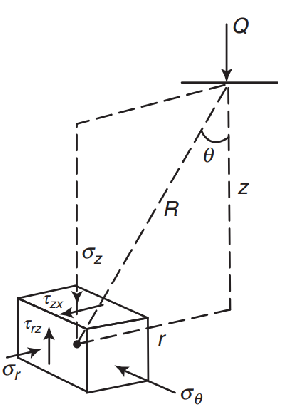
\includegraphics[width=0.3\textwidth]{Graficos/Carga_puntual.PNG}
    \caption{Esfuerzo vertical en un punto bajo una carga puntual.}
    \label{fig:incremento_esfuerzo_vertical}
\end{figure}
El código de este caso se encuentra en el siguiente link: \href{https://github.com/berckanala/Fundaciones_P2/blob/main/Codigos/python/esfuerzo_puntual.py}{Código esfuerzo puntual}
En donde:
\begin{itemize}
    \item $Q$: carga puntual (N)
    \item $r$: distancia radial al punto de interés (m)
    \item $z$: profundidad del punto de interés (m)
\end{itemize}

\subsubsection*{Carga Distribuida}
\begin{figure}[h]
    \centering
    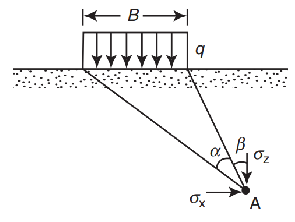
\includegraphics[width=0.4\textwidth]{Graficos/Carga_distribuida.PNG}
    \caption{Esfuerzo vertical en un punto bajo una carga distribuida.}
    \label{fig:distibuido_esfuerzo_vertical}
\end{figure}

El código de este caso se encuentra en el siguiente link: \href{https://github.com/berckanala/Fundaciones_P2/blob/main/Codigos/python/esfuerzo_distribuida_externa.py}{Código esfuerzo carga distribuida externa}\\
En donde:
\begin{itemize}
    \item $q$: carga distribuida (N/m)
    \item $a$: distancia entre la carga y el punto de interes (m)
    \item $z$: profundidad del punto de interés (m)
    \item $B$: longitud de la carga distribuida (m)
\end{itemize}
En cuantos a la carga distribuida interna, el código se encuentra en el siguiente link: \href{https://github.com/berckanala/Fundaciones_P2/blob/main/Codigos/python/esfuerzo_distribuido_interna.py}{Código esfuerzo carga distribuida interna}\\
En donde:
\begin{itemize}
    \item $q$: carga distribuida (N/m)
    \item $z$: profundidad del punto de interés (m)
    \item $B$: longitud de la carga distribuida (m)
\end{itemize}

\subsubsection*{Distribución rectangular uniforme}
Para este método, dependiendo de donde se encuentre el punto de interés, se debe dividir la fundación en partes iguales. Por ejemplo, si el punto es en el centro de la fundación, se divide en 4 partes iguales, y si el punto de interés es a un lado de la fundación, se divide en 2 partes iguales, como se muestra a continuación:
\begin{figure}[h]
    \centering
    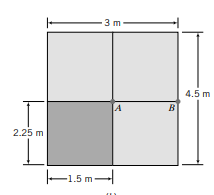
\includegraphics[width=0.4\textwidth]{Graficos/distribucion_rectangular.PNG}
    \caption{Esfuerzo vertical en un punto bajo una carga distribuida rectangular uniforme.}
    \label{fig:distribucion_rectangular}
\end{figure}
Para poder calcular el esfuerzo en el punto A, se divide en 4 partes iguales, y se calcula el esfuerzo en cada una de las partes, y luego se suman los esfuerzos. Mientras que en el punto B, se divide en 2 partes iguales, y se calcula el esfuerzo en cada una de las partes, y luego se suman los esfuerzos. \\
El código de este caso se encuentra en el siguiente link: \href{https://github.com/berckanala/Fundaciones_P2/blob/main/Codigos/python/incremento_tensiones.py}{Código esfuerzo carga distribuida rectangular uniforme}\\
\newpage

\subsubsection*{Distribución circular uniforme}
\begin{figure}[h]
    \centering
    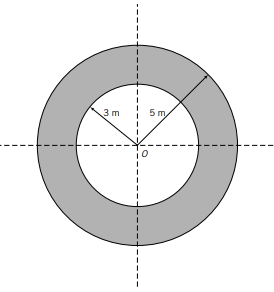
\includegraphics[width=0.4\textwidth]{Graficos/Carga_circular.PNG}
    \caption{Esfuerzo vertical en un punto bajo una carga distribuida circular uniforme.}
    \label{fig:distribucion_circular}
\end{figure}

El código de este caso se encuentra en el siguiente link: \href{https://github.com/berckanala/Fundaciones_P2/blob/main/Codigos/python/esfuerzo_circular.py}{Código esfuerzo carga distribuida circular uniforme}\\

\subsubsection*{Terraplen}

\begin{figure}[h]
    \centering
    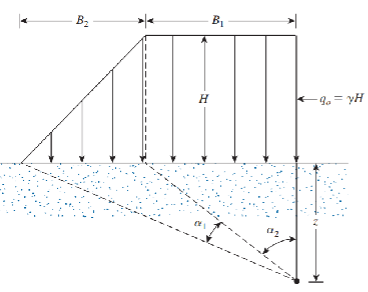
\includegraphics[width=0.6\textwidth]{Graficos/Carga_terraplen.PNG}
    \caption{Esfuerzo vertical en un punto bajo una carga distribuida de terraplen.}
    \label{fig:terraplen}    
\end{figure}

Este código se encuentra en el siguiente link: \href{https://github.com/berckanala/Fundaciones_P2/blob/main/Codigos/python/esfuerzo_terraplen.py}{Código esfuerzo terraplen}\\
En donde:
\begin{itemize}
    \item $q$: carga distribuida (N/m)
    \item $z$: profundidad del punto de interés (m)
    \item $B1$: longitud de la base del terraplen (m)
    \item $B2$: longitud de la carga triangular (m)
\end{itemize}

\section{Asentamiento de la fundación}


\subsection*{Tipos de asentamientos en arenas}
\begin{itemize}
    \item \textbf{Asentamiento inmediato (elástico)}
    \item \textbf{Asentamiento consolidado (primaria)}: Es instantánea
    \item \textbf{Asentamiento secundario}: Es muy baja en general
\end{itemize}
\subsection*{Tipos de asentamientos en arcillas}
\begin{itemize}
    \item \textbf{Asentamiento inmediato (elástico)}: Tería elástica
    \item \textbf{Asentamiento consolidado (primaria)}: Consolidación
    \item \textbf{Asentamiento secundario}: Creep
\end{itemize}

En arcillas también se presentan asentamientos elásticos.
Sin embargo, los asentamientos por consolidación primaria son los más
significativos y se estiman a través de la teoría de consolidación de
Terzaghi. Además, para estimar la consolidación es necesario conocer los
parámetros Cc y Cs, los cuales se obtienen del ensayo de tensión-
deformación en el Odómetro.

\subsection*{Forma general}
Según la forma general se ocupan 2 ábacos:

\begin{figure}[h]
    \centering
    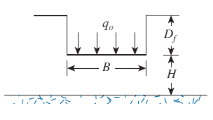
\includegraphics[width=0.5\textwidth]{Graficos/asentamiento_3.PNG}
    \caption{Figura de asentamiento.}
    \label{fig:asentamiento1}
\end{figure}

Se tiene que utilizar la siguiente fórmula para poder calcular el asentamiento:
\[
S_e = A_1 \cdot A_2 \frac{q_0 B}{E_s}
\]


\begin{itemize}
    \item $S_e$: Asentamiento elástico (m)
    \item $A_1$: Coeficiente de asentamiento (m)
    \item $A_2$: Coeficiente de asentamiento (m)
    \item $q_0$: Carga aplicada (kN/m2)
    \item $B$: Ancho de la fundación (m)
    \item $E_s$: Módulo de elasticidad del suelo (kN/m2)
\end{itemize}
\newpage
A continuación se presentan los ábacos de asentamiento A1 y A2, que son:

\begin{figure}[h]
    \centering
    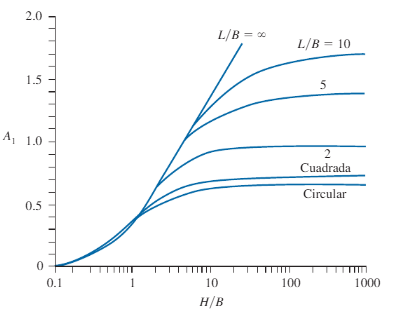
\includegraphics[width=0.5\textwidth]{Graficos/asentamiento_2.PNG}
    \caption{Ábaco de asentamiento A1.}
    \label{fig:asentamiento2}
\end{figure}


\begin{figure}[h]
    \centering
    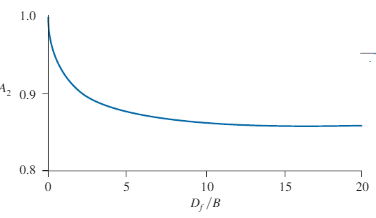
\includegraphics[width=0.5\textwidth]{Graficos/asentamiento_1.PNG}
    \caption{Ábaco de asentamiento A2.}
    \label{fig:asentamiento3}
\end{figure}

Además, de la teroría elástica, se sabe que:

\[
\Delta l = \frac{q \alpha B}{E}
\]
Donde $\alpha$ es el coeficiente de asentamiento, que depende del tipo de suelo y de la carga aplicada.\\


\end{document}